\documentclass[12pt]{article}

\usepackage{graphicx}

\title{AMath Tea Time --- Puzzle \#1}
\author{}
\date{\vspace{-1cm}31 March 2015}

\begin{document}

\maketitle
\pagenumbering{gobble}

{\it Hello, everyone! I thought it would be nice to have weekly
  mathematical and programming puzzles to accompany our tea time
  activities. My plan is to post new puzzles every Tuesday and add
  hints on Thursday. Discuss solutions with others and have fun!

  --

  Chris S.}

\subsection*{Problem}

There are 2015 airports in the far away land of Dijkstrania. Every
pair of airports is connected by a nonstop flight in one or both
directions. Show that there is some airport from which it is possible
to reach every other airport in at most two flights.

\begin{figure}[hb]
  \centering
  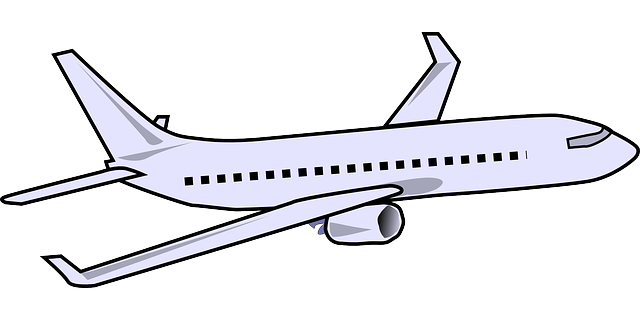
\includegraphics[width=0.4\textwidth]{airplane.png}
\end{figure}

\subsection*{Hints}

{\it (Posted on Thursday)}


{
\par\vspace*{\fill}
\noindent \small \it
If you have any puzzles to share then send them my way at {\tt
  cswiercz@uw.edu}!
}

\end{document}
